% Options for packages loaded elsewhere
\PassOptionsToPackage{unicode}{hyperref}
\PassOptionsToPackage{hyphens}{url}
\PassOptionsToPackage{dvipsnames,svgnames,x11names}{xcolor}
%
\documentclass[
  letterpaper,
  DIV=11,
  numbers=noendperiod]{scrartcl}

\usepackage{amsmath,amssymb}
\usepackage{iftex}
\ifPDFTeX
  \usepackage[T1]{fontenc}
  \usepackage[utf8]{inputenc}
  \usepackage{textcomp} % provide euro and other symbols
\else % if luatex or xetex
  \usepackage{unicode-math}
  \defaultfontfeatures{Scale=MatchLowercase}
  \defaultfontfeatures[\rmfamily]{Ligatures=TeX,Scale=1}
\fi
\usepackage{lmodern}
\ifPDFTeX\else  
    % xetex/luatex font selection
\fi
% Use upquote if available, for straight quotes in verbatim environments
\IfFileExists{upquote.sty}{\usepackage{upquote}}{}
\IfFileExists{microtype.sty}{% use microtype if available
  \usepackage[]{microtype}
  \UseMicrotypeSet[protrusion]{basicmath} % disable protrusion for tt fonts
}{}
\makeatletter
\@ifundefined{KOMAClassName}{% if non-KOMA class
  \IfFileExists{parskip.sty}{%
    \usepackage{parskip}
  }{% else
    \setlength{\parindent}{0pt}
    \setlength{\parskip}{6pt plus 2pt minus 1pt}}
}{% if KOMA class
  \KOMAoptions{parskip=half}}
\makeatother
\usepackage{xcolor}
\setlength{\emergencystretch}{3em} % prevent overfull lines
\setcounter{secnumdepth}{-\maxdimen} % remove section numbering
% Make \paragraph and \subparagraph free-standing
\ifx\paragraph\undefined\else
  \let\oldparagraph\paragraph
  \renewcommand{\paragraph}[1]{\oldparagraph{#1}\mbox{}}
\fi
\ifx\subparagraph\undefined\else
  \let\oldsubparagraph\subparagraph
  \renewcommand{\subparagraph}[1]{\oldsubparagraph{#1}\mbox{}}
\fi


\providecommand{\tightlist}{%
  \setlength{\itemsep}{0pt}\setlength{\parskip}{0pt}}\usepackage{longtable,booktabs,array}
\usepackage{calc} % for calculating minipage widths
% Correct order of tables after \paragraph or \subparagraph
\usepackage{etoolbox}
\makeatletter
\patchcmd\longtable{\par}{\if@noskipsec\mbox{}\fi\par}{}{}
\makeatother
% Allow footnotes in longtable head/foot
\IfFileExists{footnotehyper.sty}{\usepackage{footnotehyper}}{\usepackage{footnote}}
\makesavenoteenv{longtable}
\usepackage{graphicx}
\makeatletter
\def\maxwidth{\ifdim\Gin@nat@width>\linewidth\linewidth\else\Gin@nat@width\fi}
\def\maxheight{\ifdim\Gin@nat@height>\textheight\textheight\else\Gin@nat@height\fi}
\makeatother
% Scale images if necessary, so that they will not overflow the page
% margins by default, and it is still possible to overwrite the defaults
% using explicit options in \includegraphics[width, height, ...]{}
\setkeys{Gin}{width=\maxwidth,height=\maxheight,keepaspectratio}
% Set default figure placement to htbp
\makeatletter
\def\fps@figure{htbp}
\makeatother

\KOMAoption{captions}{tableheading}
\makeatletter
\makeatother
\makeatletter
\makeatother
\makeatletter
\@ifpackageloaded{caption}{}{\usepackage{caption}}
\AtBeginDocument{%
\ifdefined\contentsname
  \renewcommand*\contentsname{Table of contents}
\else
  \newcommand\contentsname{Table of contents}
\fi
\ifdefined\listfigurename
  \renewcommand*\listfigurename{List of Figures}
\else
  \newcommand\listfigurename{List of Figures}
\fi
\ifdefined\listtablename
  \renewcommand*\listtablename{List of Tables}
\else
  \newcommand\listtablename{List of Tables}
\fi
\ifdefined\figurename
  \renewcommand*\figurename{Figure}
\else
  \newcommand\figurename{Figure}
\fi
\ifdefined\tablename
  \renewcommand*\tablename{Table}
\else
  \newcommand\tablename{Table}
\fi
}
\@ifpackageloaded{float}{}{\usepackage{float}}
\floatstyle{ruled}
\@ifundefined{c@chapter}{\newfloat{codelisting}{h}{lop}}{\newfloat{codelisting}{h}{lop}[chapter]}
\floatname{codelisting}{Listing}
\newcommand*\listoflistings{\listof{codelisting}{List of Listings}}
\makeatother
\makeatletter
\@ifpackageloaded{caption}{}{\usepackage{caption}}
\@ifpackageloaded{subcaption}{}{\usepackage{subcaption}}
\makeatother
\makeatletter
\@ifpackageloaded{tcolorbox}{}{\usepackage[skins,breakable]{tcolorbox}}
\makeatother
\makeatletter
\@ifundefined{shadecolor}{\definecolor{shadecolor}{rgb}{.97, .97, .97}}
\makeatother
\makeatletter
\makeatother
\makeatletter
\makeatother
\ifLuaTeX
  \usepackage{selnolig}  % disable illegal ligatures
\fi
\IfFileExists{bookmark.sty}{\usepackage{bookmark}}{\usepackage{hyperref}}
\IfFileExists{xurl.sty}{\usepackage{xurl}}{} % add URL line breaks if available
\urlstyle{same} % disable monospaced font for URLs
\hypersetup{
  colorlinks=true,
  linkcolor={blue},
  filecolor={Maroon},
  citecolor={Blue},
  urlcolor={Blue},
  pdfcreator={LaTeX via pandoc}}

\author{}
\date{}

\begin{document}
\ifdefined\Shaded\renewenvironment{Shaded}{\begin{tcolorbox}[sharp corners, frame hidden, interior hidden, borderline west={3pt}{0pt}{shadecolor}, breakable, enhanced, boxrule=0pt]}{\end{tcolorbox}}\fi

\hypertarget{conclusions-and-future-work}{%
\section{Conclusions and Future
Work}\label{conclusions-and-future-work}}

\hypertarget{sec-conclusions}{%
\subsection{Conclusions}\label{sec-conclusions}}

\hypertarget{general-overview}{%
\subsubsection{General Overview}\label{general-overview}}

I started writing this thesis with one broad aim \(-\) to couple insect
odorant receptors with either a carbon nanotube or graphene field-effect
transistor for highly selective sensing in the vapour phase. Through
this process, I hoped to gain new physical insights into the transducer
and receptor elements used, through careful examination of the
biosensors which resulted from their coupling. At the end of this
investigation, three broad themes have emerged:

\begin{itemize}
\item
  Slight variations in transducer morphology have a substantial impact
  on biosensor sensitivity and power consumption.
\item
  Intrinsic transducer hysteresis leads to biosensor current drift,
  which can be modelled and corrected for when interpreting sensing
  data.
\item
  Surface contamination can affect transducer functionalisation and lead
  to significant variability in biosensor quality.
\end{itemize}

These findings and their relation to the goal of creating a reliable
biosensor for a vapour-phase detection system are each detailed in this
section.

\hypertarget{biosensor-performance-and-transducer-morphology}{%
\subsubsection{Biosensor Performance and Transducer
Morphology}\label{biosensor-performance-and-transducer-morphology}}

Carbon nanotube networks and graphene are used as the thin-film for
sensing field-effect transistors due to their highly sensitive surface.
However, particular features present on each film may enhance or reduce
the sensitivity of the transistor. They may also affect the power
required to maximise device sensitivity. The process used for randomly
depositing carbon nanotubes influences multiple aspects of the resulting
network morphology, including the density and homogeneity of the
network, the diameter of bundled carbon nanotubes, the level of doping
present and the relative proportion of metallic to semiconducting
nanotubes. These variables were investigated atomic force microscopy,
Raman spectroscopy and electrical characterisation. Devices with carbon
nanotubes deposited using surfactant in the presence of steam were found
to have relatively dense and homogeneous networks which gave rise to
highly consistent electrical characteristics, desirable for biosensor
reproducibility and multiplexing. Carbon nanotube bundle diameters were
also much smaller in these networks, which gave them a relatively large
on-off ratio and subthreshold slope, figures of merit which correspond
to low power operation. However, steam-assisted surfactant-deposited
devices were found to have significant \(p\)-doping, possibly from
surfactant. Removing the source of this \(p\)-doping would further
enhance the sensitive and low power performance of these devices.

\hypertarget{biosensor-drift-and-transducer-hysteresis}{%
\subsubsection{Biosensor Drift and Transducer
Hysteresis}\label{biosensor-drift-and-transducer-hysteresis}}

All devices characterised showed a degree of hysteresis, which was
especially significant for solvent-deposited carbon nanotube network
devices as well as any device when backgated. This hysteresis is a
result of the evolving occupancy of charge traps, which are introduced
to the device by gate bias or adsorbed dopants. This changing occupancy
leads to a slow drift in current level when the transistor is operated
with constant voltages at both the drain and gate. If left until
reaching a steady state, this baseline drift can be modelled using a
linear combination of three exponentials. However, it is not feasible to
wait more than three hours for a biosensor to warm up with each use. A
series expansion was used to model the drift over a shorter period of
time, where the two longer time constant exponentials were approximated
as linear. This meant only having to wait until the first exponential
had decayed before sensing, which typically took \textless30 minutes for
a pristine, liquid-gated steam-deposited carbon nanotube device. Each
exponential term may correspond to charge traps introduced at different
stages of fabrication and functionalisation. For example, long-term
drift was consistent across channels fabricated simultaneously, but
appeared to be affected by functionalisation.

\hypertarget{biosensor-functionalisation-and-transducer-contamination}{%
\subsubsection{Biosensor Functionalisation and Transducer
Contamination}\label{biosensor-functionalisation-and-transducer-contamination}}

\begin{itemize}
\item
  threshold voltage shift compares gating behaviour of devices
\item
  most functionalisation procedures used to attach odorant receptors are
  non-covalent
\item
  more consistent limit of detection for covalent attachment
\item
  all vapour sensing with nanodiscs has used covalent functionalisation
\item
  non-specific binding: misoriented attachment, substrate attachment\\
\item
  non-covalent functionalisation \(-\) \(\sim\) 7 ppb by Goldsmith
  \emph{et al.}
\item
  AFM evidence for adsorped water vapour and/or surfactant, long
  histogram tail more than 5 nm in height
\item
  Raman evidence for adsorped water vapour and/or surfactant,
  \(I_{D}/I_{G}\) ratio increased for steam-assisted surfactant
  deposited device
\item
  graphene devices seen to be slightly \(p\)-doped from their rightwards
  shifted major Dirac point, could be adsorbed photoresist
\item
  steam-assisted surfactant-deposited devices heavily \(p\)-doped,
  average \(V_t\) = 0.37 V relative to \(V_t\) = 0.27 V for
  solvent-deposited, could be resist, steam adsorption or surfactant
  residue
\item
  devices shown to be sensitive to PBS additions (electrostatic gating)
  and adsorption of vapour, however direct charge transfer may not be
  involved!!! just because a device is sensitive does not mean it is
  clean and functionalisable
\item
  unclear whether dense PBASE surface coverage is desirable, possible
  that the use of an excessive PBASE or PBA concentration leads to
  multilayer coverage which reduces the quality of functionalisation
\end{itemize}

-MeOH and DMSO can both be adsorbed to the channel, causing a change in
transfer characteristics due to capacitive gating

\begin{itemize}
\item
  Raman and pyrene-PEG-FITC fluorescence microscopy showed that pyrene
  linker was attaching to the channel
\item
  PEG or pyrene-PEG often used for the prevention of non-specific
  binding
\item
  biomolecules will preferentially stick to residual resist over the
  channel if not sufficiently hardbaked, shown with fluorescence
  microscopy
\item
  long-chain alkanes from air make channel hydrophobic and repel
  functionalisation material in aqueous solution, can be removed with
  low power plasma
\end{itemize}

-non-specific binding occurs between pyrene-based linker and the
SiO\(_2\) substrate

\begin{itemize}
\item
  variability in successful functionalisation seen for iOR biosensors
  using the standard PBASE in methanol method, PBASE and nanodiscs
  attach but do not significantly gate the network
\item
  possible coatings originally included surfactant, solvent,
  photoresist, multilayered or hydrolysed PBASE, and hydrophobic
  long-chain alkanes, all were eliminated by sensing experiments until
  only alkane hydrocarbons, multilayer linker attachment and photoresist
  were left as possibilities
\item
  oxygen plasma cleaning was unreliable due to impact on mobility
\item
  no response for vapour sensing, either needs covalent
  functionalisation with protective membrane or capture layer
\end{itemize}

\hypertarget{sec-future-work}{%
\subsection{Future Work}\label{sec-future-work}}

\hypertarget{sec-future-work-fabrication}{%
\subsubsection{Device Fabrication and
Functionalisation}\label{sec-future-work-fabrication}}

\hypertarget{improved-encapsulation}{%
\paragraph*{Improved Encapsulation}\label{improved-encapsulation}}
\addcontentsline{toc}{paragraph}{Improved Encapsulation}

Ceramic encapsulation with HfO\(_2\) (see ceramic encapsulation paper)

Need special SU8 as SU8-2150 and AZ\(^\circledR\) 1518 photoresist both
fluoresce

use previous OR fluorescence test paper with PEG and GFP-ORs to check
for successful passivation of SiO\(_2\)

could also use PEG-FITC and GFP-ORs to check for passivation of
unmodified carbon nanotubes (without GFP-ORs)

\hypertarget{surface-contamination}{%
\paragraph*{Surface Contamination}\label{surface-contamination}}
\addcontentsline{toc}{paragraph}{Surface Contamination}

Could model surface contamination using a linear combination of normal
or skew-normal distributions {[}@Marchenko2010{]}. Alternatively, could
improve microscopy and get closer to normal distribution by altering the
force applied by microscope tip {[}@Vobornik2023{]}.

Thermal oxidation {[}@Kane2014; @Barnett2018{]}, cleaning with oxygen
radicals {[}@Petkov2005{]}

\hypertarget{covalent-approaches}{%
\paragraph*{Covalent Approaches}\label{covalent-approaches}}
\addcontentsline{toc}{paragraph}{Covalent Approaches}

\begin{itemize}
\tightlist
\item
  use of Cu2+/AB-NTA (Nα,Nα-Bis(carboxymethyl)-L-lysine hydrate) with
  diazonium salt used to functionalise single carbon nanotube for
  detection of eugenol vapour in real-time {[}@Goldsmith2011{]}
\end{itemize}

NTA chelates with metal ions, with a particularly strong bond to
Cu\(^{2+}\) {[}@Chang2017{]}

\begin{itemize}
\item
  use of antibody fragments
\item
  systematic comparison of the effectiveness of different covalent
  techniques (quality of functionalisation vs channel mobility
  post-functionalisation)
\end{itemize}

\hypertarget{investigating-or-orco-complex}{%
\paragraph*{Investigating OR-ORCO
Complex}\label{investigating-or-orco-complex}}
\addcontentsline{toc}{paragraph}{Investigating OR-ORCO Complex}

\begin{itemize}
\item
  Lim \emph{et al.} {[}@Jin2012; @Park2012a; @Lim2014; @Lim2015;
  @Son2015; @Ahn2015{]} but with ORCO ion channel and iOR in liposomes
  instead of Kir potassium ion channel and hOR
\item
  Could try using sodium, calcium and potassium ions just as the ORCO
  channel does \emph{in vivo}, (also VUAA1), gives a better idea of the
  behaviour and role of ORCO {[}@Wicher2021{]}
\item
  are other intracellular components or ion channels required for
  operation??
\end{itemize}

\hypertarget{multiplexing}{%
\paragraph*{Multiplexing}\label{multiplexing}}
\addcontentsline{toc}{paragraph}{Multiplexing}

A scent in nature contains a mixture of many different volatile organic
compounds in vapour at different concentrations. A major goal for a
vapour-phase iOR biosensor is therefore to perform multiplexed
measurements with different iORs in different channels to simultaneously
measure and distinguish between mixtures of volatile organic compounds
{[}@Kwon2015; @Hurot2020; @Hirata2021{]}. A similar approach could be
taken to that of Kwon \emph{et al.} and Son \emph{et al.}, but for
insect odorant receptors {[}@Kwon2015; @Son2017{]}. A difficulty that
could arise here is that iORs may specifically bind with multiple VOCs.
When interacting with an iOR, different volatiles can `antagonise' each
other; some iORs will not respond to a positive ligand if another
specific ligand is present {[}@Kwon2015; @Munch2016; @Son2017;
@Hirata2021{]}. This means a multiplexed iOR biosensor would first need
to be tested individually against different volatile compounds, and then
with mixtures of volatile compounds to detect any antagonistic
behaviours in a systematic manner. Care should be taken to avoid the
coffee-ring effect when functionalising individual channels of a device
(\textbf{?@sec-coffee-ring}). The use of small, deep microchannels in
clean PDMS, which keep functionalisation material close to the channel,
may be essential for consistent functionalisation.

\hypertarget{sec-future-work-vapour}{%
\subsubsection{Vapour Sensing}\label{sec-future-work-vapour}}

\hypertarget{flow-system}{%
\paragraph*{Flow System}\label{flow-system}}
\addcontentsline{toc}{paragraph}{Flow System}

Replace all three mass flow controllers with two MFCs with maximum flow
both equal to either 1000 or 10000 sccm. One MFC should be kept at a
constant flow rate through the dilution line at all times during a
sensing experiment. The other should also be kept at a constant flow
rate at all times, but feed into a computer-automated solenoid valve
which is able to switch the flow between multiple lines. Under normal
operation, this second MFC should also be directed through the dilution
line. During a sensing series, it should then be redirected through the
carrier line.

More consistent, used by Goldsmith \emph{et al.}

May need to replace PVC with stainless steel tubing, introduce a vapour
trap to the system before the vacuum pump for use with more corrosive
volatile compounds able to significantly degrade PVC at low
concentrations

\hypertarget{capture-layer}{%
\paragraph*{Capture Layer}\label{capture-layer}}
\addcontentsline{toc}{paragraph}{Capture Layer}

Insect odorant receptors are stabilised by having their lipid membrane
maintained in an aqueous environment. Exposing iORs to vapour-phase
compounds outside this environment may cause them significant damage
without the use of a protective membrane protein {[}@Sato2014;
@Warden2019{]}. A capture layer can be used to mimic the mucus within
the insect sensillum lymph, which protects the dendrite cells
{[}@Sato2014; @Hurot2020; @Cali2020; @Shkodra2021{]}. This capture layer
could also be used as a liquid-gate to maximise device sensitivity. A
gate electrode can be photolithographically patterned onto the device
surface alongside the source and drain electrodes for this purpose,
making contact with the capture layer through an additional gap in the
device encapsulation {[}@Shkodra2021{]}. Only slight alterations would
have to be made to the device design outlined in this thesis for
implementation.

A variety of possible capture layer solutions for vapour-phase
field-effect transistor sensors can be found in the literature. Lee
\emph{et al.} and Kuznetsov \emph{et al.} integrated an aqueous membrane
held by polycarbonate and SiO\(_2\)/Si\(_3\)N\(_4\)/SiO\(_2\) into their
sensor, which prevented electrolyte evaporation {[}@Lee2015;
@Kuznetsov2018{]}. Bio-gels or ionic liquids (ILs) are other potential
candidates. Sato \emph{et al.} used an agarose hydrogel in a
microchamber array as a capture layer {[}@Sato2014; @Hirata2021{]}.
Ionic liquids have low vapour pressure, high capacitance, as well as
high electrochemical stability. Hwang \emph{et al.} and White \emph{et
al.} used 1-Butyl-3-methylimidazolium bis(trifluoromethylsulfonyl)imide
(BMIM) as the electrolytic gate for thin-film field-effect transistors
{[}@Hwang2014; @White2015{]}. Alternative ionic liquid candidates may
need to be identified which are biologically compatible.

A potential difficulty with this approach might be ensuring rapid
odorant diffusion through the layer to the iOR-FET surface, especially
when compounds are insoluble {[}@Pelosi2018; @Warden2019; @Cali2020;
@Hurot2020; @Yamada2021; @Spencer2021{]}. Yamada \emph{et al.} used
hydrophobic microslits at the liquid-vapour interface to promote mixing
of compounds within an aqueous environment {[}@Yamada2021{]}. It may
also be possible to use odorant binding proteins to carry volatile
compounds to the odorant receptors, just as \emph{Drosophilia
Melanogaster} does \emph{in vivo} {[}@Larisika2015; @Brito2016;
@Sankaran2011; @Kotlowski2018; @Pelosi2018; @Cali2020{]}.

\#\#\#\# Multiplexing \{.unnumbered\}

\begin{figure}

{\centering 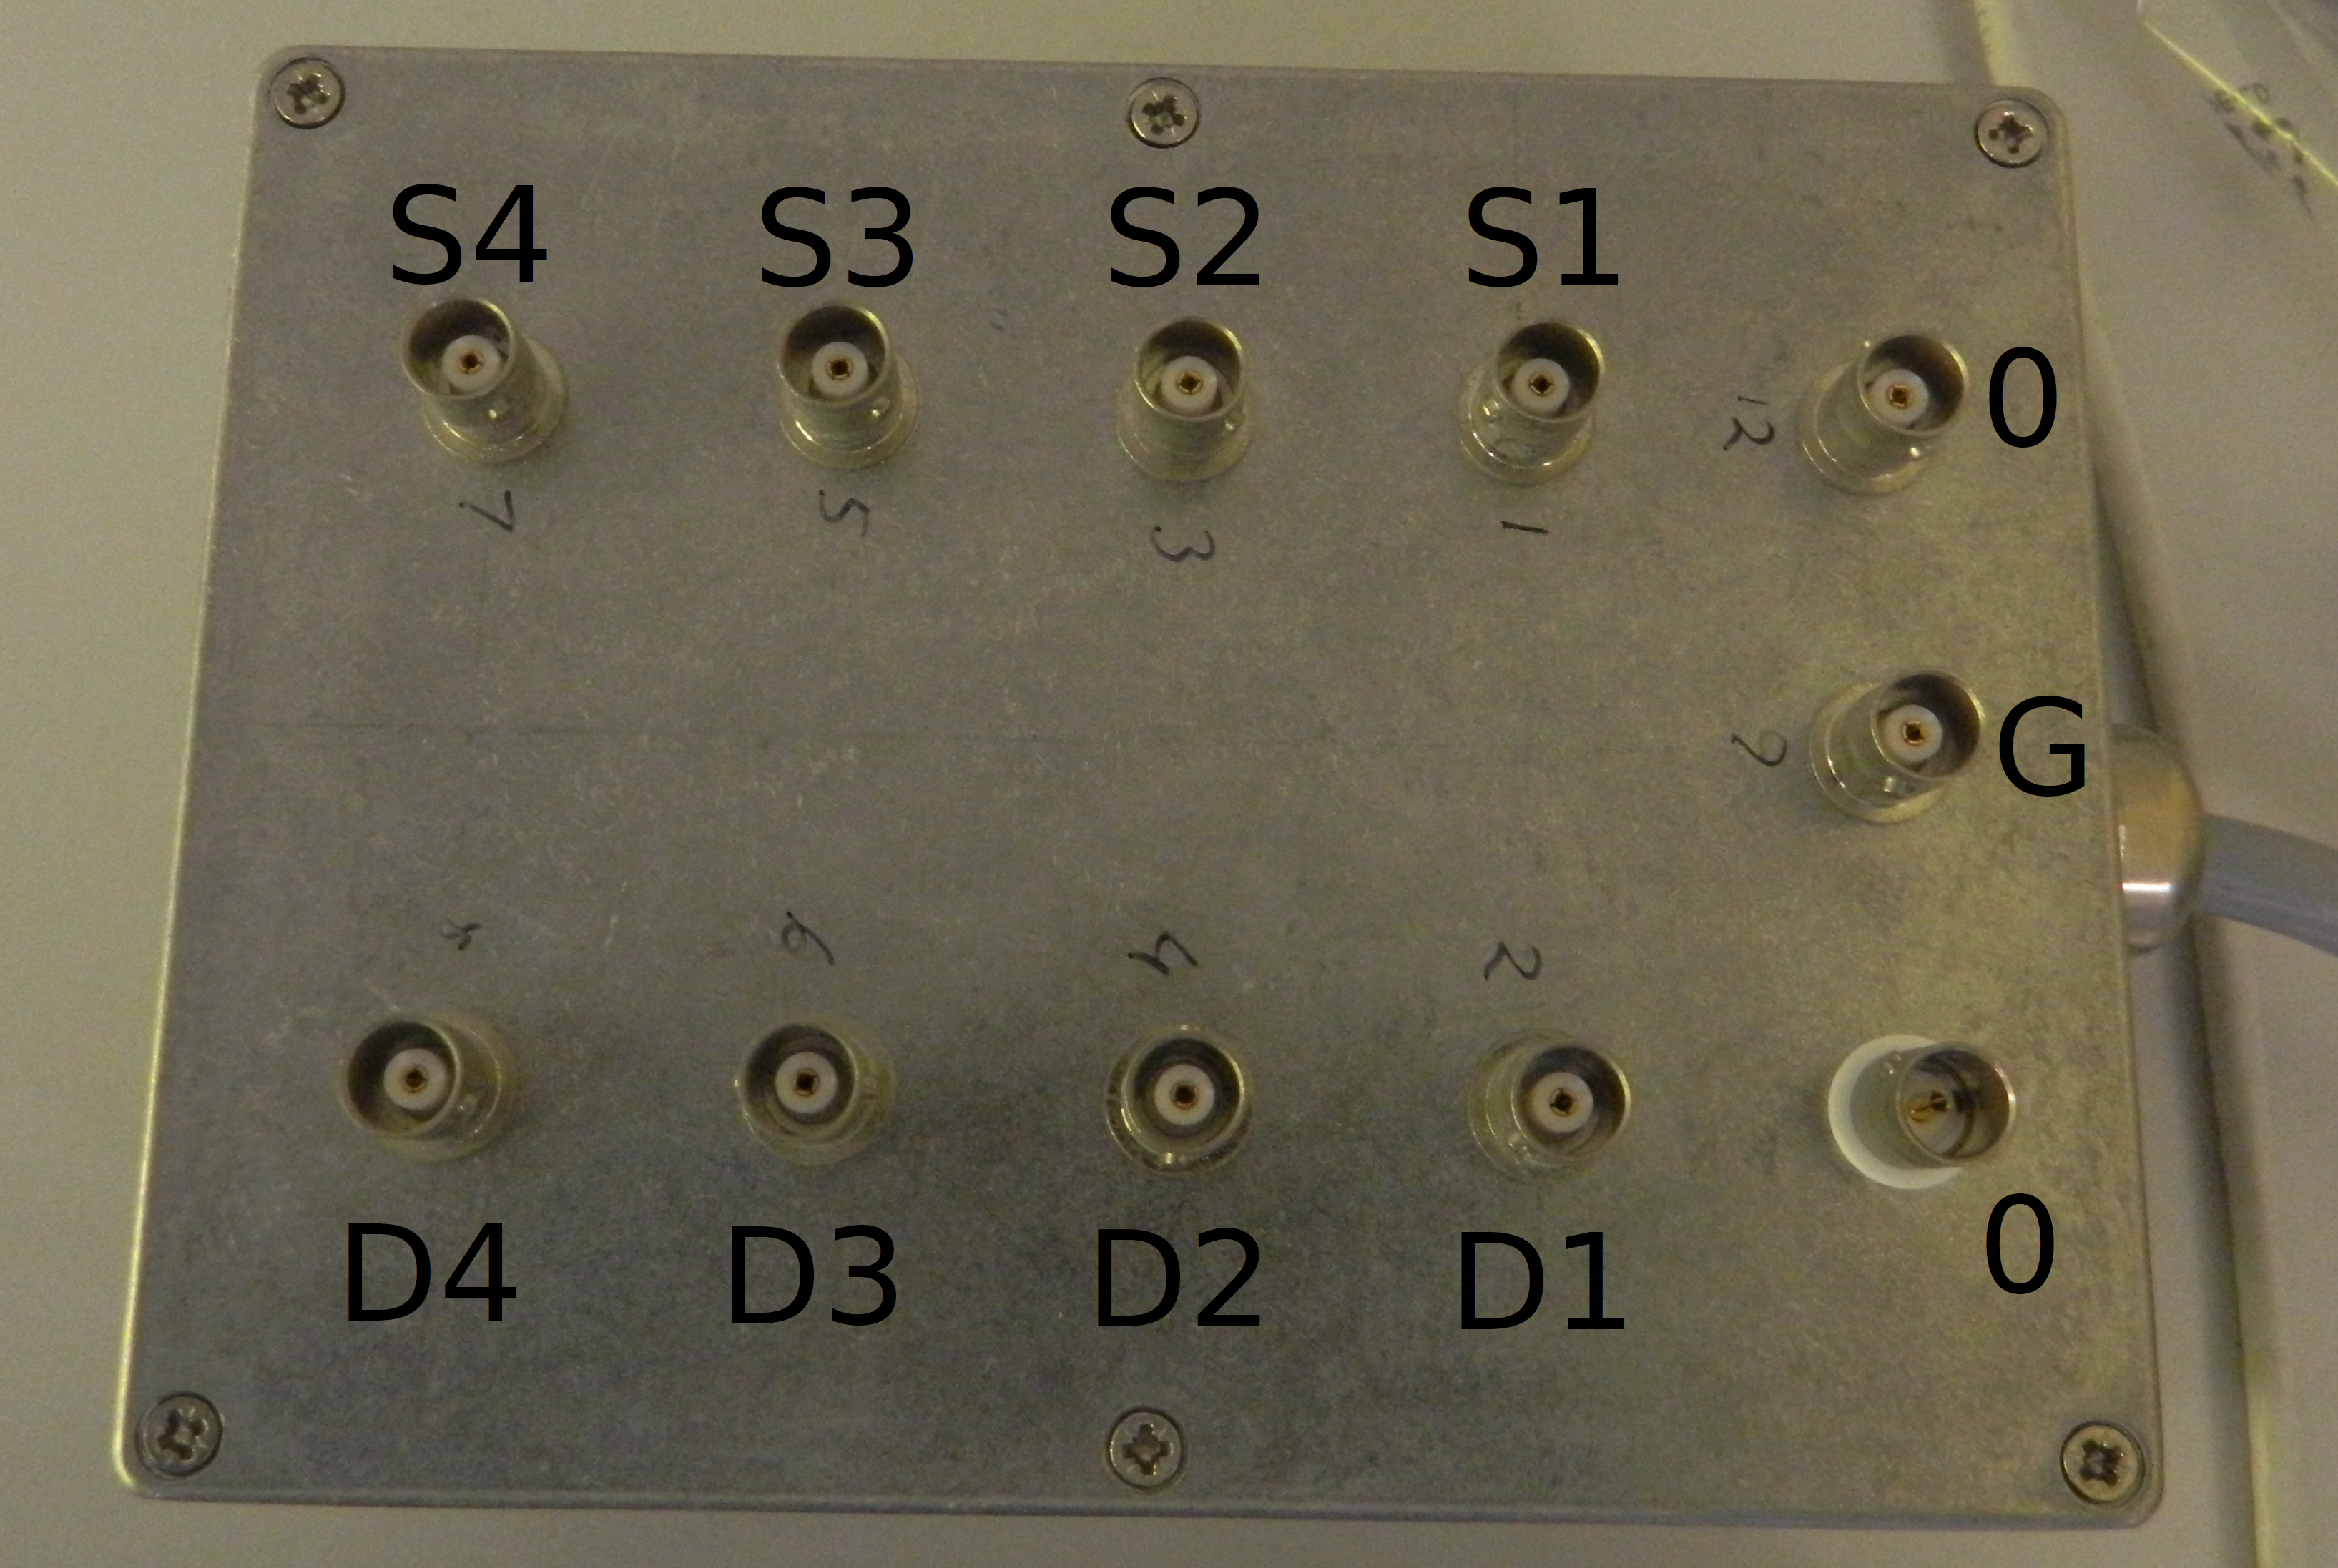
\includegraphics{figures/ch9/multiplex-breakout.png}

}

\caption{\label{fig-vapour-sensor-breakout}Breakout board for vapour
delivery system device. Source electrode terminals are labelled S, drain
electrode terminals are labelled D, the gate electrode terminal is
labelled G and disconnected terminals are labelled 0. Each number
corresponds to a different device channel.}

\end{figure}

already possible to connect four channels at once through custom
breakout board, sufficient to test three ORs simultaneously alongside
empty ORs

\includegraphics{figures/ch9/multiplex-vapoursensor.png}\{\#fig-vapour-sensor
multiplexing\}

Install a second analyte bottle branching off from the existing carrier
line, place 4-way valve after analyte bottles which runs one analyte
bottle to exhaust and one to chamber

Can alternate between analyte and nitrogen with flow through the analyte
bottle, and therefore the amount of vapour passing out of the bottle,
largely unchanged across a sensing run

Can alternate between two analytes (control analyte and response
analyte) with flow through each uninterrupted

Each carrier line only ever contains one analyte, to prevent
cross-contamination between lines.

With a 16-way or 32-way valve, more analyte bottles could be added and
therefore multiplexing with more ORs in a single experimental run



\end{document}
